% !TEX encoding = UTF-8 Unicode

%!TEX TS-program = xelatex
%!TEX encoding = UTF-8 Unicode

\documentclass[oneside,12pt]{book}
\usepackage[left=2cm,top=1cm,right=3cm,nofoot]{geometry}                % See geometry.pdf to learn the layout options. There are lots.
\geometry{a4paper}                   % ... or a4paper or a5paper or ... 
\usepackage{tabularx}

\usepackage{fontspec,xltxtra,xunicode}
\defaultfontfeatures{Mapping=tex-text}
\usepackage[french]{babel}
\usepackage{listings}
\usepackage{graphicx}
\usepackage[linktocpage]{hyperref}
\newcommand\don[5]{
\textbf{#1} \\
#2
\begin{itemize}
\item{ \textbf{jet}: #3}
\item{ \textbf{Cout}: #4}
\item{ \textbf{Page}: #5}
\end{itemize}
\vspace{0.5cm}
}


\title{Traditions Ecossaisses}
\author{Renaud "ObiWan" Guezennec}
\date{}

%\let\origdescription\description
%\renewenvironment{description}{
%  \setlength{\leftmargini}{0em}
%  \origdescription
%  \setlength{\itemindent}{1em}
%}


\begin{document}

\maketitle \clearpage
\tableofcontents \clearpage

\begin{flushleft}
    \chapter{Introduction}
        \section{Lire introduction sur l'univers de loup-garou}
       Les loup-garou sont mi-humain mi-esprit de loup. Il y a très longtemps dans une époque qu'il surnomme la Pangée, Père loup faisait régner l'ordre entre le monde physique et le monde des esprits.\\ Devant son courage, Mère Lune tomba amoureuse de père loup. Elle pris forme humaine pour le séduire. Elle donna naissance à 9 enfants (les premiers nés). De Mère lune ils reçurent la faculté de changer de forme et Père-Loup la force et l'instinct de chasseur. Au fils des siècles, après la naissance de plusieurs générations de loup-garou, le pouvoir de père loup perdit de sa vigueur, diluer dans ses enfants et les enfants de ses enfants. Une partie des enfants de Père loup réalisa qu'il était trop faible pour les guider, ils proposèrent leur aide mais Père-loup refusa. Alors ses enfants assassinèrent Père loup  qui refusait de partager son fardeau avec le fruit de sa chair. Lorsque le coup mortel fut porté, Pere-loup cria si fort qu'il déchira le monde. Depuis lors, le monde des esprits (hisile) est éloigné du monde physique. Les esprits en veulent au loug garou (uratha) car ils ont cassé leur paradis et on réussi là où ils avaient tous échoué (tuer père loup). Mère lune maudit ses propres enfants pour leur crime. Depuis, les loup garou sont sensible à argent (le metal le plus précieux au yeux de Mere Lune). Au fil des siècles, elle pardonna, en partie, aux loup-garous qui reprirent le travail de son bien aimé. Le respect de l'équilibre entre le monde des esprits et le monde physique est donc la responsabilité des Loup-garou. \\
Le monde des esprits est un monde où il fait toujours nuit. Chaque élément du monde physique a son reflet dans l'autre monde à l'exception des humains. Les humains nourrissent par leurs émotions le monde des esprits. Les esprits peuvent être des concept comme la violence, la jalousie l'appétit ou bien des objets esprit d'une porte d'un animal. Les loup-garous sont les seuls êtres autorisé à passer d'un monde à l'autre. \\
Le loug garou peut à volonter se transformer entre 5 formes.\\ 
Locus\\
Régénération\\
Les ennemis :\\
-Les esprits : leur but est de grandir le plus possible,\\ 
-Les purs : Loup garous qui refusèrent de prendre par à la mort de Père-Loup\\
Les ligues sont des mouvements philosophiques chez les loup garou.\\


\subsection{Serment de la Lune}
Les loups doivent chasser\\
Le peuple ne tue pas le peuple\\
Le faible honore le fort, Le fort respecte le faible.\\
Respecte ta proie\\
Le peuple doit vivre parmi les humains.\\
Ne mange pas de chair humaine ou de loup.\\
Le troupeau ne doit pas savoir.      \\


\section{Les meutes déchues}
\subsection{La Meute PJ: }
A définir, mais un nombre important de personnage doit être présent à la reconstitution. 

\subsection{La meute badass : Brook children}
Ils seront tous morts au début du scénario. Ils passaient pour des gros guerriers mais c'est plus de la frime.


\section{Les meutes Pures}
\subsection{La Meute PJ: les mercyless claw}
Allan McGuire \\


\clearpage
\chapter{Les personnages Joueurs}
\clearpage
\section{Elodothe}
\begin{description}
\item[Nom:]{Allan McGuire}
\item[Origine:]{Ecosse}
\item[Tribu:]{Maitre du fer}
\item[Profession:]{Emploie dans une association}
\item[liste don:]{demi lune,perspicacité, protection, modelage, savoir, technologie}
\item[Nom de guerre:]{Hammer Of Law}
\item[Age:]{22}
\item[Histoire:]{ 
    Tu es un ancien étudiant en droit, tu travailles pour une association de protection des droits qui aide les gens dans le besoin: femmes battues, droits des étrangers..\\
    Tu es salarié, cela ne paye pas des masses mais tu aimes aider les gens. Tes compétences de droit aide beaucoup, la majorité de ta promo est en passe de devenir avocats ou juge.\\ C'est ta nouvelle condition qui ta poussé à travailler. Concilier la vie d'un loup-garou et celle d'un étudiant n'est pas évident. Le travail dans l'association est te permet d'avoir tes horraires.  \\
C'est pendant tes études que tu es devenue loup garou, à la suite de cette transformation.\\
    Tu as préféré t'isoler un peu et travailler seul. Le gros de ton boulot est principalement lire les textes des nouvelles lois, écrire aux élus, aider des gens pour leur papier. \\
 Monter des dossiers de révision de dossier/procès. tu bosses de chez toi, cela te laisse pas mal de temps pour la meute. 
Lors d'une manifestation contre l'augmentation des frais de scolarité à la fac, tu as vu un policier anti émeutes frapper à coup de mattraque une pauvre étudiante avec des béquilles. Tu t'es interposé et tu as été améné au poste. Les flics ont voulu se faire de l'étudiant, pas de chance pour eux, ils s'en sont pris à un loup-garou en devenir. Tu as réussi à t'enfuir, pour te reveiller le lendemain matin complètement nu sur un toit. \\ 
Dans la presse, un article évoquait la mort de 3 agents dans leur fourgon. Tu as réussi à rentrer chez toi puis tu as fait profil bas. Puis tu as rencontré Julia, tu as dessuite senti qu'elle était comme toi.\\ 
Vous avez aussi remarqué que votre nouvelle condition attiré tout un tas de chose étrange autour de vous. Ensemble c'était plus facile de réagir face à ces nouveautés. \\

Focus est une personne de confiance, vous vous entendez très bien. Ce n'est pas la même chose avec Joker qui est trop individualiste à ton gout. Il est un bon élément dans la meute mais en tant qu'humain tu le trouves un peu mauvais. 
Doctorius est un peu trop concentré sur ses recherches, il devrait prendre une plus grande par dans la vie de la meute.  
Tonic est une femme forte et triste. Elle a vécu un grand traumatisme lors de son premier changement. 
}
\end{description}
\clearpage
\textbf{\large Dons} 
\vspace{0.5cm}

\don{Voir sous la surface}{sentir la duperie}{astuce + empathie + pureté vs calme + instinct primal}{1 point de volonté}{112}
\don{Aura de treve}{projette aura de calme}{manipulation + persuasion + honneur}{1 ESSENCE}{113}
\don{Nuit noire}{éteindre les lumières sur 200m² par succès}{Astuce + Larcin + Ruse}{1 volonté}{146}
\don{Redresser}{redresse un objet }{}{1 essence}{125}

\clearpage
\section{Cahalithe}
\begin{description}
\item[Nom:]{Julia Andrews}
\item[Origine:]{Ecosse}
\item[Auspice:]{Cahalithe}
\item[Tribu:]{Griffe de Sang}
\item[Profession:]{Journaliste}
\item[Nom de guerre:]{Focus}
\item[Liste de dons:]{inspiration,Lune gibbeuse, Savoir, Force, Rage}
\item[Age:]{24}
\item[Histoire:]{
Journaliste indépendante et blogeuse, tu publies pas mal d'article sur les politiques véreux, pots de vins etc. Cela t'a value des ennuies. 
Virée de la fac de journaliste après avoir publier des photos du directeur avec son neuve. Il t'arrive de vendre des articles pour des médias étrangers sur tel ou tel évènement.\\ 
C'est au cours d'une filature d'un homme politique, que tu es devenu loup garou. Ses hommes de mains se sont montrés un peu entreprenant, ils ne pourront plus jamais le faire. Ce fut sale. Tu t'es réveillé (nue), sans comprendre ce qui s'était passé. Tu es rentrée chez toi. C'est à partir de ce moment que tes rêves ont commencé.\\
Des territoires étranges lugubres et tristes. Tu as mis du temps à avant de sortir de chez toi après ces évènements. Puis tu as rencontré Allan (Hammer of Law) qui était visiblement dans la même situation que toi.\\
Vous avez vite compris qu'a deux vous étiez plus fort face aux nouvelles menaces. Les créatures de tes rêves semblait de plus en plus proche de toi. 
Puis vous avez trouvé les autres. D'autres loup garou vous ont trouvé et expliqué un peu la situation et votre raison de vivre. Vous avez pris pour territoire le sud de Stirling. \\

Ce soir, grace à ta carte de presse, tu as un siège réservé à la tribune pour assister à la commémoration de la bataille de Stirling. Tu seras en plein milieu du gratin de la ville et de l'écosse. \\
Les autres membres de la meute vont faire partie du spectacle. \\
Tu as révé de cris d'enfant, tu sais que tu as de temps en temps des rêves prémonitoires. Des cris tristes et de colères, vraiment étrange cela n'avait rien d'humain. \\

Hammer est un homme bien, peut-être un peu trop lié à son travail. Il est cepandant un bon chef et sait écouter.
Joker est un mec viril, c'est assez important dans la meute, il est toujours pour l'action mais sait quand c'est trop dangereux.
Tonic est un femme virile, elle est très belle mais aussi très forte. Tu jalouses un peu son style.
Doctorius est marrant il est tout le temps plongé dans ses livres et devrait sortir un peu, il a été bien utile à la meute.
}
\end{description}
\clearpage
\textbf{\large Dons} 
\vspace{0.5cm}

\don{coup fracacant}{Dégats lethaux à la place de contondants(scène)}{}{1 volonté}{116}
\don{saut puissant}{+6 dés pour faire un saut}{}{}{116}
\don{Les bons mots}{+2 en social passif}{}{}{117}
\don{Connaitre un nom}{Permet d'apprendre le ou les noms auxquels  le personnage répond}{Intelligence + Investigation + ruse vs Résolution + Instinct Primal}{}{144}


\clearpage
\section{Irraka}
\begin{description}
\item[Nom:]{Edward MacClur}
\item[Origine:]{Ecosse}
\item[Auspice:]{Irraka}
\item[Tribu:]{Seigneur des tempêtes}
\item[Profession:]{Petite frappe}
\item[surnom:]{Joker}
\item[liste de don:]{Discrétion, Evasion, Nouvelle lune, Domination, Evasion, météorologie}
\item[Age:]{29}
\item[Histoire:]{
Personnage charismatique, tu es l'atout charme de ta meute. Tu es un fin commercial et un grand manipulateur. \\ 
En plus de cela tu n'es pas le dernier en ce qui concerne
la baston. 
Pour vivre tu fais un peu de tout: trafic de drogue, faux papiers, armes, braquages, tu peux aussi faire des trucs plus légaux mais c'est moins fun.\\
Tu es bien conscient que ton "travail" ne plait pas beaucoup auprès des autres membres de la meutes. Cela reste un bon moyen pour rester indépendant.\\
Tu aimes cette liberté, tu sais qu'avec ta meute tu es plus puissant cependant cela te plait de parcourir la ville dans l'ombre. Il ne faut pas oublié que tes connaissances sont très utiles pour ta meute. Tu es au courant des gros coups. Tu es aussi un indic de la police. Tu vends généralement des infos pas très fraiche mais cela te fait un complément de revenu. \\
Alors que tu rentrés du stade, tu as croisé la route d'hooligans, ils t'ont attaqué avec des battes, barres à mines.. Tu as réussi à t'enfuir dans le parc, blessé tu t'es caché sous un banc public. Le lendemain matin, tu t'es révéillé complètement nu dans le parc. Heureusement Julia est venue à ta rencontre.\\
Tu as intégré sa meute. Tu restes le vilain petit canard à cause de ton "travail".\\

L'alpha reste le plus farouche adversaire envers toi. Il est un bon chef mais trop jeune à ton gout. Tu prendras sa place un jour. Il faut juste que tu gagnes les soutiens des autres. 
Focus est marrante, elle comprend un peu les raisons qui t'ont poussé à devenir ce que tu es.
Tu admires un peu Doctorius, ses connaissances sont impressionnantes. Tu aurais aimé devenir comme lui. 
Tonic est sympa mais un peu trop sérieuse parfois. Elle refuse que tu vendes ta merde dans son bar. Cependant tu as droit à pas mal de conso gratuite. C'est super cool ça.  


}
\end{description}
\clearpage
\textbf{\large Dons} 
\vspace{0.5cm}



\don{Ombre mouvante}{Deplacement silencieux}{}{1 essence}{115}
\don{langue délié}{faire parler quelqu'un}{manipulation + entregent + Sagesse vs Calme + instinct primal}{1 essence}{110}
\don{s'esquiver}{se libérer de menottes, cordes, porte, camisole...}{}{1 volonté}{112}
\don{Brouillard silencieux}{}{}{}{123}

\clearpage
\section{Ithaeur}
\begin{description}
\item[Nom:]{Jack Humsteal}
\item[Origine:]{Gallois}
\item[Auspice:]{Ithaeur/shaman}
\item[Tribu:]{Os de L'ombre}
\item[Profession:]{étudiant en histoire}
\item[Surnom:]{Doctorius}
\item[Liste de dons:]{Croissant de Lune, Element, Modelage, Mort, perspicacité, Protection}
\item[Age:]{19}
\item[Histoire:]{
Étudiant sérieux, tu as toujours été un bon élève. Passionné par les anciennes cultures et les légendes, tu es venu en Écosse pour faire une licence d'histoire. 
Hélas, c'est à cette période que tu es devenu un loup garou. Les premiers signes furent des faims énormes ou bien des envies de violence. Cela ne te resemblait pas. Tu étais en boite de nuit et un mec a fait chier ta copine de l'époque (tu te souviens même plus de son prénom). Tu t'es battu avec lui, il a gagné cela ta énervé et tu as commencé à te transformer. \\
Tu t'es reveillé le lendemain dans une pièce noire, sans aucune sortie. Après quelques heures, une certaine Alice s'est présenté à toi. Quelques choses en elle te mettait mal à l'aise. Elle t'a appris qu'elle était comme toi un être surnaturel mais pas du même genre. Tu es un loup-garou c'est une vampire très ancienne. Elle t'a caché de la foule (t'empechant de faire un massacre). Tu es resté avec elle quelques temps puis tu as compris que ta place était avec d'autres loups garous. Tu as rejoins la meute. Le temps passé avec Alice a augmenté ta soif de savoir occulte. \\

Dans la meute, tu es le shaman. \\

Focus et Hammer sont les membres fondateurs de la meute, ils prennent leur role de loup garou trop au sérieux. Ils sont fatiguant.
Joker est plus marrant, il sait se marrer lui, plus que toi en tout cas. C'est pour cela que tu l'admires. Il est souvent utile pour se changer les idées.
Tonic te fait peur. Tu l'as vu se battre, c'est un pur monstre. Tu fais bien attention de ne pas la contredire. Elle reste cependant assez cool avec toi et te charie un peu (amicalement). \\

}
\end{description}
\clearpage
\textbf{\large Dons} 
\vspace{0.5cm}


\don{Vision de mort}{voir les troubles laisser par les fantômes}{}{}{104}
\don{oeil sur les deux mondes}{voir dans les deux mondes en même temps}{Astuce + occulte + Sagesse}{}{127}
\don{Témoignage de cadavre}{le mort racconte ce qu'il a vu depuis sa mort}{Manipulation + Occulte + Pureté}{}{129}

\textbf{\large Rituels} 
\vspace{0.5cm}
\don{Funéraire}{}{}{}{151}
\don{convoquer un esprit}{}{}{}{152}


\clearpage
\section{Rahu}
\begin{description}
\item[Nom:]{Jessica Martin (MacHalligan)}
\item[Origine:]{Ecosse}
\item[Auspice:]{Rahu}
\item[Tribu:]{chasseur des ténébres}
\item[Profession:]{barman}
\item[Surnom:]{Tonic}
\item[liste don:]{domination, force, pleine lune,discretion, elements, nature}
\item[mots clés:]{grande, indépendante, utopiste blazée}
\item[Age:]{26 ans}
\item[Histoire:]{ 
Issue d'une famille très riche d'écosse, tu as toujours vécu dans le luxe. Tes parents avaient arrangé une union avec le fils d'une autre famille. Tu avais été préparé à cela toute ta vie. Au premier regard, ton prétendant était un homme charmant, cepandant quand vous vous etes retrouvé seul, tu as vite compris qu'ils serait risqués. sans avoir vraiment peur de lui, car tu sais te défendre, il te considérait comme une marchandise dont il pouvait disposer. Lors d'une promenade en forêt dans tes domaines. Il a essayé de te violer. Essayer seulement car tu t'es transformé à ce moment là. Ce ne fut pas propre. Le lendemain matin, tu te reveilla couverte de sang. \\ 
Celle nuit là, tu as tué ton prétendant, sa soeur cadette, ta mère et le gardien des parcs de ta famille. Ton père étant mort, il y a longtemps (cancer des poumons).    tu as hérité de la fortune, l'enquête a conclu à l'attaque d'une meute de loup ou de chien (les loups ne sont plus présent en grande bretagne donc cela reste bizarre comme explication, mais les blessures correspondaient à cela).\\
Depuis cet évènement, tu as pris une nouvelle identité. Tu as toujours assez à la forturne familliale mais cela tu ne le souhaites pas. En te cherchant un nouveau but, tu as rencontré Allan (Hammer of Law) et Julia (la journaliste). Tu as aidé la meute à s'installer en achetant un bar dans le sud de Stirling. C'est le centre de votre territoire et votre locus.\\

Hammer est un type bien, encore jeune et plein d'illusions sur les humains. 
Focus reste une fille intéressante, couragueuse et débrouillarde, tu es un peu jalouse car elle est ce que tu ne seras jamais une "fille sans problème". 
Joker se prend pour un type intéressant, il fait son job mais sa soif de pouvoir ou de reconnaissance est un véritable problème.
Doctorius est un type sérieux mais ses fréquentations sont bizarres, il se pourrait qu'elles l'emmene à agir contre la meute.
}
\end{description}
\clearpage
\textbf{\large Dons} 
\vspace{0.5cm}


\don{Clarté}{+5 en initiative}{}{1 essence}{137}
\don{Volonté de Luna}{}{présence + intimidation + Gloire vs Calme + Instinct Primal}{}{107}
\don{Diriger le feu}{}{Force + Survie + Gloire}{1 essence}{109}
\don{Langue animale}{Parler avec un animal (1 mins par succès)}{Manipulation + Animaux + Pureté}{1 essence}{130}

\chapter{La vérité: MJ}
\section{Informations aux PJ}
\begin{itemize}
\item[à definir]: à définir
\end{itemize}

\section{Nom des meutes}
\begin{itemize}
\item[Mercyless Claws]: meute de purs jeune
\item[Clever Knights]: 
\item[Brook Children]: tous morts
\end{itemize}


\section{C'est la Fête!}
L'écosse vient d'obtenir son indépendance du royaume-uni. Cela provoque dans toute l'écosse un regain de patriotisme. Les gens font la tournée des bars en kilt en chantant.
Le vote a été fait, il y a 3 jours. L'anniversaire de la bataille de Stirling sera le bouquet final de la célébration. Comme chaque année, une reconstitution de la bataille est organisé. 


\section{La meute des Purs}
Le territoire est situé au nord du lieu de la bataille. Les troupes écossaisses se sont installées sur leur territoire et preparent la reconstitution.

\section{La meute des déchus}
Le territoire est situé au sud du lieu de la bataille. Les troupes anglaises se sont installées sur leur territoire et preparent la reconstitution.


\section{La meute des Inconnus}
Le territoire de cette meute est le lieu précis de la bataille, il est suit le court de la rivière.
Il reste très mystérieux, on rendu des services des deux côté. Ils sont extrèmement puissant. Leur territoire est un gros locus de victoire et de violence. 
Leur totem est un cheval de guerre (persévérence et force). 


\section{Les territoires}
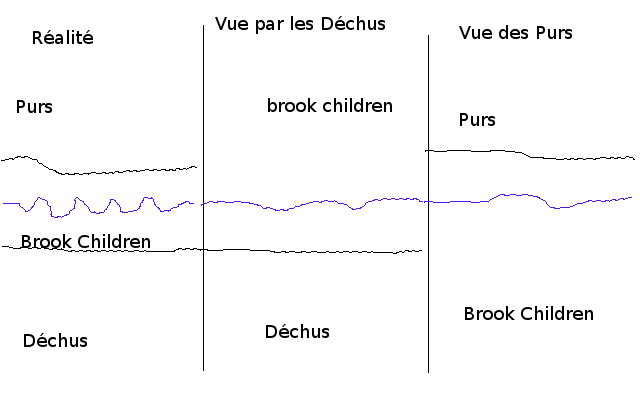
\includegraphics[scale=0.5]{schemaPurDechu.png} \\

L'idée du scénario double est que chaque meute de joueur pense que l'autre table joue les "Brook children". Il sera plus facile de garder cet intrigue pour les déchus qui n'enquêteront pas sur le décés de loup garou.

Les brook children ont tjs fait croire au meute voisine qu'il possédé un grand territoire.

\section{Edward McAllister dit «Sad Howl»}
Loup garou à la recherche de son frère jumeau.
C'est un déchus, il est mort, tué par une partie de la meute des Brook Children. 


\section{Brook Children}
Ils sont des loup garou très porté sur la ruse. Ce sont des Déchus mais aucun membre n'avait de réel puissance martiale.
Ils se font passer pour des purs au près de la meute des mercyless Claws. ce sont des déchus et leur territoire est assez petit. Cependant il font croire qui est énorme. 
La rivière est leur totem. Leur locus est le lieu de la bataille de Stirling. C'est deux gros avantages. 
2 de leur membre sont des cerbères qui travaille pour un esprit de la corruption. Ils ont été poussé a se reproduire pour mettre au monde un enfant fantôme.
L'accouchemen a tué la mère, quand le reste de la meute a compris, ils ont chassé le père (le frère de Edward McAllister (Sad Howl)). Ils ont tué son frère, on continué la chasse et son mort tué par l'enfant fantome. 


\section{Unihar : Enfant fantome}
Pur esprit, très difficile à tuer (voir ses stats ). Il est le serviteur d'un esprit de la corruption. il cherche a tuer tous les loup garou dans la zone.\\

Rank: 4\\
Attributes: Power 12, Finesse 12, Resistance 11\\
Willpower: 23\\
Essence: 25\\
Initiative: 23\\
Defense: 12\\
Speed: 34\\
Size: 6\\
Corpus: 17\\
Influences: Uratha ••, Hatred ••\\
Numina: Discorporation, Gauntlet Breach, Harrow, Howl*,\\
Material Vision, Rage Armor†, Revelation*, Sense Weakness†,
Speed*\\
Bans: While they are cunning enough to bide their time
and grow strong enough to accomplish their goal, unihar
are almost always held under a ban to exact revenge. Their
primary targets are usually their parents, although some
are driven to seek revenge on all werewolves and some
also against the humans and/or wolves who embody the
unihar’s absent corporeal side.\\
Special: Ghost Children are immune to all werewolf Gifts
and rites, as well as the effects of fetishes that duplicate
such Gifts or rites’ effects. This immunity does not extend
to certain byproducts of a werewolf’s powers — for example,
a spear formed through a Shaping Gift would affect a
Ghost Child in the same way that a mundane spear would.\\
However, even Gifts that redirect existing phenomena
to strike the Ghost Child (such as Command Fire) cannot
directly target the unihar.\\

\section{Idigam : Esprit de la corruption}
Par le biais de son nouveau toutou, il veut tuer tous les loup garou pour pouvoir venir dans ce lieu. La création de la lésion est une des étapes pour sa venue.

\section{Magath : Esprit de l'argent/pouvoir}
Il est un peu fou dans sa tête. L'idigam l'a corrumpu pour le forcer à influncer des êtres humains.

\section{Le riche donnateur}
influencé par le magath, il s'est arrangé pour que le campement écossais recoive des vraies épées en manipulant le maire. 
Le forgeron du camp a eu un cadeau très puissant pour éguiser les épées. quant l'idigam n'a plus eu besoin de lui, Unihar est venu le tuer ainsi que l'esprit d'argent.






\chapter{Scénario pour les Purs}

A définir. 


\section{l'enquete des purs}
Les purs vont découvrir les corps de la meute des enfants de la rivière. 
Dans un premier temps, ils trouverons le corps d'une femme avec le bas totalement déchiré (la mère).



\section{}

\section{La découverte des corps}
Les deux meutes vont retrouver les corps de la meute
 
\subsection{Parler avec le totem}
Il leur dira qu'il est temps pour eux d'agrandir leur territoire. Il peut parler du territoire de vente. Danger mais plus de puissance.

\subsection{Le deal}
Les purs ont rendez-vous avec un gang pour un echange d'armes/droges. Interventions des flics au loin.

\subsection{Le Pub}
Si les joueurs sont invité a rejoindre leur locus (pub) ultra conservateur. Ils y a des troubles. 
C'est maintenant qu'ils appennent le drame par les infos. 

\subsection{Le Totem}
Le totem contacte la meute, il est temps pour eux de prendre l'avantage sur la meute voisine.


\subsection{les esprits.}





\chapter{Scénario pour les Déchus}

\section{Rituel funéraire}
La meute accomplie le rituel funéraire pour un loup garou nomade mort sur leur territoire. 
Il s'était présenté sous le nom de «Sad Howl» (Triste hurlement), il y a quelques jours pour demander la permission d'entrer sur le territoire. Il a été tué sur leur territoire (à la frontière). 

Note au Mj: Ce petit chapitre donne le ton du scénario, il est important que les jours fasse leur tour de table des description. Insister sur le coté triste et sur la description du rituel.


\section{Le carnage de Stirling}
Certains membres de la meute vont etre acteur de la reconstitution. Pendant la bataille, ils peuvent être en contact avec des lames en argents.
A la discretion du MJ pour la pureté de l'argent si pur => dégat aggravé et test de rage mortelle, sinon cela chauffe au contact.
(Voir déroulement de la bataille) 
Faire quelques jets de combats, faire attention aux armes utilisés.  Une lésion est né sur la bataille. 

\section{Les secours}
 Les secours arrivent après plusieurs heures de combats. Les victimes évacuées.
C'est le bon moment de présenter un ou deux PNJ important, un inspecteur de police, un medecin (il demandera à controler les blessures, s'ils ont été blessé à l'argent
la cicatrice est vraiment impressionnante, il demandera à l'étudier encore plus). 
C'est une scene de RP importante. 

\section{L'enquête}
La presence de l'argent va surement réveiller la curiosité des loup garous.
Le monde des esprits est saturé d'esprits de violence, de mort (bref s'ils vont la-bas les esprits les attaques à vue).
Il y a de nombreux fantômes sur le lieux de la bataille. (Il pourrait être amusant que certains fantome soit la depuis la vrai bataille de Stirling, pour ajouter
plus de confusion chez les joueurs, Le vrai fantôme répètera "Independance pour l'écosse" et des trucs comme ça, si les pj lui apprennent que c'est fait, il disparait). 
Les fantomes restent assez vague dans leur dialogue cependant ils arriveront à apprendre le nom du "fabriquant". A noter que peut de fantome connaissent cette info car ils doivent être du coté écossais, il y a eu peu de mort. De toute façon le nom du fabriquant est écrit sur les armes. Une recherche sur internet donnera vite l'adresse


\section{le fabriquant}
L'entreprise est sur leur territoire, fabrication artisanane, 
mais bon c'est pour les touristes en vrai cela travaille plutot moderne.
La police y aura aussi jeter un coup d'oeil si les PJ traine dans l'enquete. L'information importante c'est que l'argent sur les lames fait parti de la commande
.C'était demandé.
Les ouvriers sont assez choqué, ils savaient que c'était pas normal de commander des vrais armes pour une reconstitution. 
Pour preuve, il peuvent voir le bon de commande (avec le client). Il semble que les lames n'était pas coupante, c'est sur place que quelqu'un les a éguisé (le prof d'histoire sous l'influence d'un fétiche).

Il peuvent continué dans 2 voix: Le forgeron, ou le client. Dans les deux cas, ils tomberont sur des gens influencés par des esprits.

\section{Le forgeron}
Le forgeron est un professeur d'histoire dans la vrai vie. Si les joueurs veulent lui parler, il faut le trouver car il se cache de la police. 
Sinon il peuvent obtenir des informations chez lui. Dans son ordinateur (ou agenda), il a noté tout le planning de la reconstitution et le rendez vous avec l'entreprise qui a fait les lames. (C'est pas vraiment un forgeron, il joue à etre le forgeron de camp ecossais pendant la reconstitution (il y connait rien).
Il a cependant pas mal de matos, dans son garage, il est possible de trouver des fétiches (Un jet en astuce + occulte - 2) permet de comprendre que des esprit de forge
et du travail sont enfermé dedans l'utilisateur fait forcement du bon travail. C'est le maire qui lui a donné la meute fétiche il y a quelques mois.

\section{Le maire (le client)}
Le maire de Stirling a été très gentiment invité en faire en sorte que la reconstitution soit "mémorable". 
Avec l'aide de l'organisateur, ils ont eu l'idée de prendre des lames en argent (plus brillant) et de vrai arme.
C'est le maire de la ville, il est pas facile a rencontré. 

\section{L'organisateur qui est aussi un riche donateur}
L'organisateur est introuvable, la police le recherche (radio, télé). En réalité, il est mort. Un jet en astuce + medecine permet de comprendre qu'il a été tué 
1 succès : par des armes coupante (cela peut être des griffes de loup garou)
2 succès : c'est des griffes de loup garou
3 succès : c'est légèrement trop gros pour être des giffes.
4 succès : elles sont auto infligées.

\section{Coté spirituel}
Il est possible d'identifier l'odeur d'un esprit present ici. Ils remarqueront deux odeurs. L'une est acre et lugubre. Elle rappelle de très mauvais ouvenir dans la mémoire collective des loups garous sans comprendre pourquoi. L'autre semblent plus normale. 
La première odeur disparer très rapidement (et aucun don ne peut aider à la pister). 
La deuxième maine à un esprit de l'argent. C'est plus vraiment un esprit d'argent c'est un esprit mutant (fusion d'un esprit d'argent (la monnaie) et le pouvoir. 
Il a été nourri par le riche donnateur/organisateur.
L'esprit explique au déchus que son hôte a été tué par l'esprit noir.
Il tient responsable les loup garou pour ce problème, c'est l'esprit noir qui a tout organiser, puis il l'a trahis. 
Il est vraiment traumatisé. 

\section{l'esprit noir}
Dans le monde des esprits, la tracque sera difficile car les purs risquent d'être dans la zone. 
A leur rencontre, les tables se croisent, si les choses troune à l'affrontement l'esprit de loge de la chasse fera sont apparition. C'est un grand esprit loup-garou. 

\section{Chasse ouverte}
Gros combat!!! 
Il est possible que Mère Lune interviennent par le bié de ses esprits inférieurs. 

























\end{flushleft}
\end{document}
